\documentclass[conference]{IEEEtran}
\IEEEoverridecommandlockouts
% The preceding line is only needed to identify funding in the first footnote. If that is unneeded, please comment it out.
\usepackage{polski}
\usepackage[utf8]{inputenc}
\usepackage{todonotes}

\usepackage{cite}
\usepackage{amsmath,amssymb,amsfonts}
\usepackage{algorithmic}
\usepackage{graphicx}
\usepackage{textcomp}
\usepackage{xcolor}
\def\BibTeX{{\rm B\kern-.05em{\sc i\kern-.025em b}\kern-.08em
    T\kern-.1667em\lower.7ex\hbox{E}\kern-.125emX}}
\begin{document}

\title{Skaner 3D wykorzystujący linię laserową\\}


\author{\IEEEauthorblockN{1\textsuperscript{st} Jarosław Mądry}
\IEEEauthorblockA{\textit{IARII} \\
\textit{Politechnika Poznańska}\\
Poznań, Polska \\
jaroslaw.madry@student.put.poznan.pl}
\and
\IEEEauthorblockN{2\textsuperscript{nd} Janusz Sendyk}
\IEEEauthorblockA{\textit{IARII} \\
\textit{Politechnika Poznańska}\\
Poznań, Polska \\
janusz.sendyk@put.poznan.pl}

}

\maketitle

\begin{abstract}
Dokument opisuje projekt optycznego skanera 3D wykorzystującego oświetlenie strukturalne w postaci linii laserowej. Laser generuje oświetlenie wykorzystując długośc fali równą 635nm. Skaner ten przystosowany został do umieszczenia na ramieniu robota manipulacyjnego UR-5.

\end{abstract}

\begin{IEEEkeywords}
skan, 3d, laser, laser plane, structured light
\end{IEEEkeywords}

\section{Wstęp}

Podstawa działania programu opiera się o równania pozwalające wyznaczyć położenie punktu w przestrzeni, który znajduje się na znanej płaszczyźnie na podstawie położenia względem obrazu z kamery.\\
$\underline{X}={P_k^+}\underline{x}+\lambda 
\begin{bmatrix}
    0\\
    0\\
	0\\
    1
\end{bmatrix}$\\
$\underline{p^T}({P_k^+}\underline{x}+\lambda*\underline{C})=0$
\\
przy czym:
\\
$\underline{X}$ - współrzędne punktu w przestrzeni\\
$P_k=
\begin{bmatrix}
    fx&0&cx\\
    0&fy&cy\\
	0&0&1\\
\end{bmatrix}\cdot
\begin{bmatrix}
    1&0&cx&0\\
    0&1&cy&0\\
	0&0&1&0\\
\end{bmatrix}$ - macierz parametrów kamery\\
${P_k^+}$ - pseudo odwrotna macierz kamery\\
$\underline{x}$ - współrzędne punktu na obrazie\\
$\underline{C}=
\begin{bmatrix}
    0\\
    0\\
	0\\
    1
\end{bmatrix}$ - współrzędne kamery\\
$\underline{p}^t = 
\begin{bmatrix}
    n_x\\
    n_y\\
	n_z\\
    -d
\end{bmatrix}$ - wektor płaszczyzny

Na podstawie 2 równania wyznaczana jest $\lambda$ a następnie wykorzystując pierwsze równanie położenie punktu w przestrzeni 3D.

\section{Mechanika}

W ramach realizowanego projektu wykonano uchwyt mocujący kamerę oraz laser w wymaganej konfiguracji. Projekt stworzony został w środowisku Autodesk Inventor, natomiast zaprojektowane elementy zostały wydrukowane za pomocą drukarki 3D przy zastosowaniu materiału PLA.


Podstawowymi założeniami projektu były:
\begin{itemize}
	\item zasięg tworzonego układu (20-60cm),
	\item prostota oraz szybkość wykonania/modyfikacji,
	\item dostosowanie uchwytu do ramienia tak, aby w jak najmniejszym stopniu ograniczał jego ruchy.
\end{itemize}

W niniejszym dokumencie zaprezentowane zostały 3 ujęcia modelu uchwytu w złożeniu z modelem robota (rys. \ref{fig:widok_robot_1}, \ref{fig:widok_robot_2} oraz \ref{fig:widok_robot_3}).

\begin{figure}[ht!]
	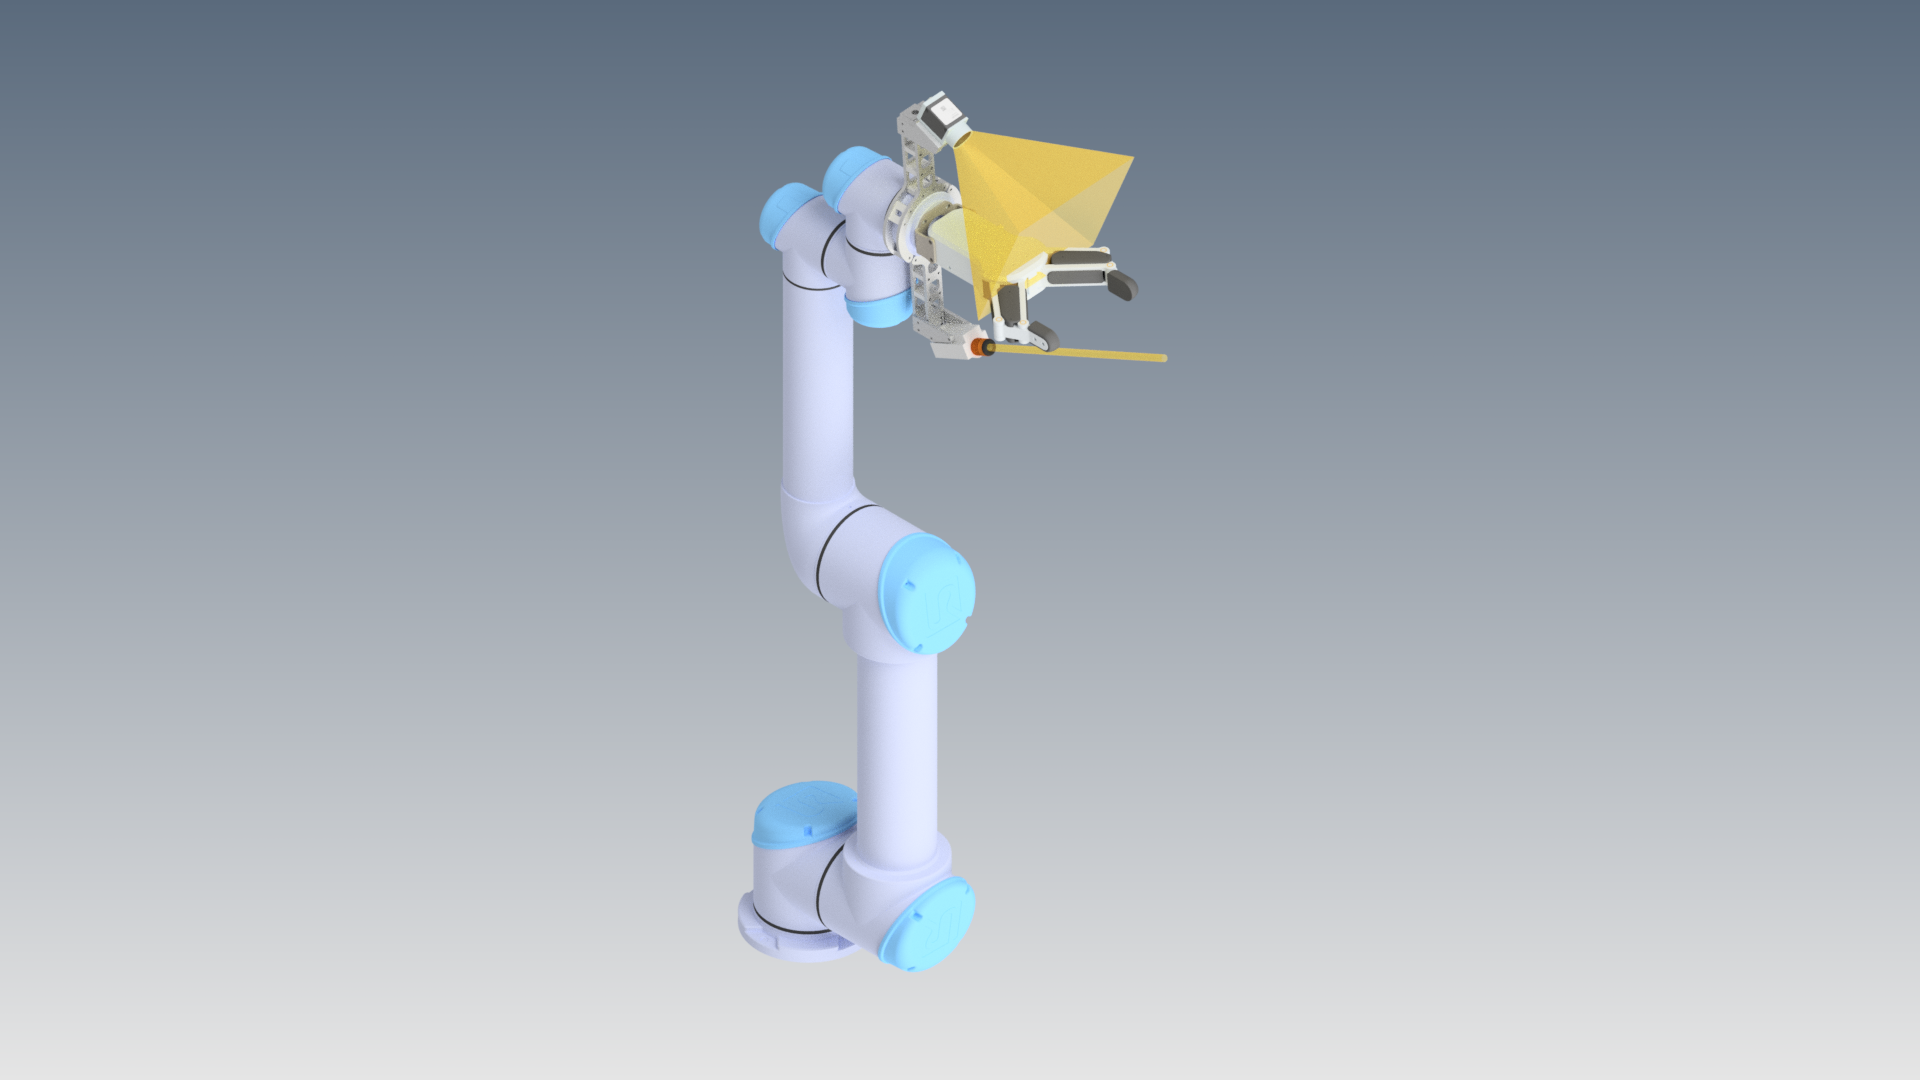
\includegraphics[width=0.45\textwidth]{figures/widok_robot_1.png}
	\centering
	\caption{Widok ogólny robota z uchwytem}
	\label{fig:widok_robot_1}
\end{figure}

\begin{figure}[ht!]
	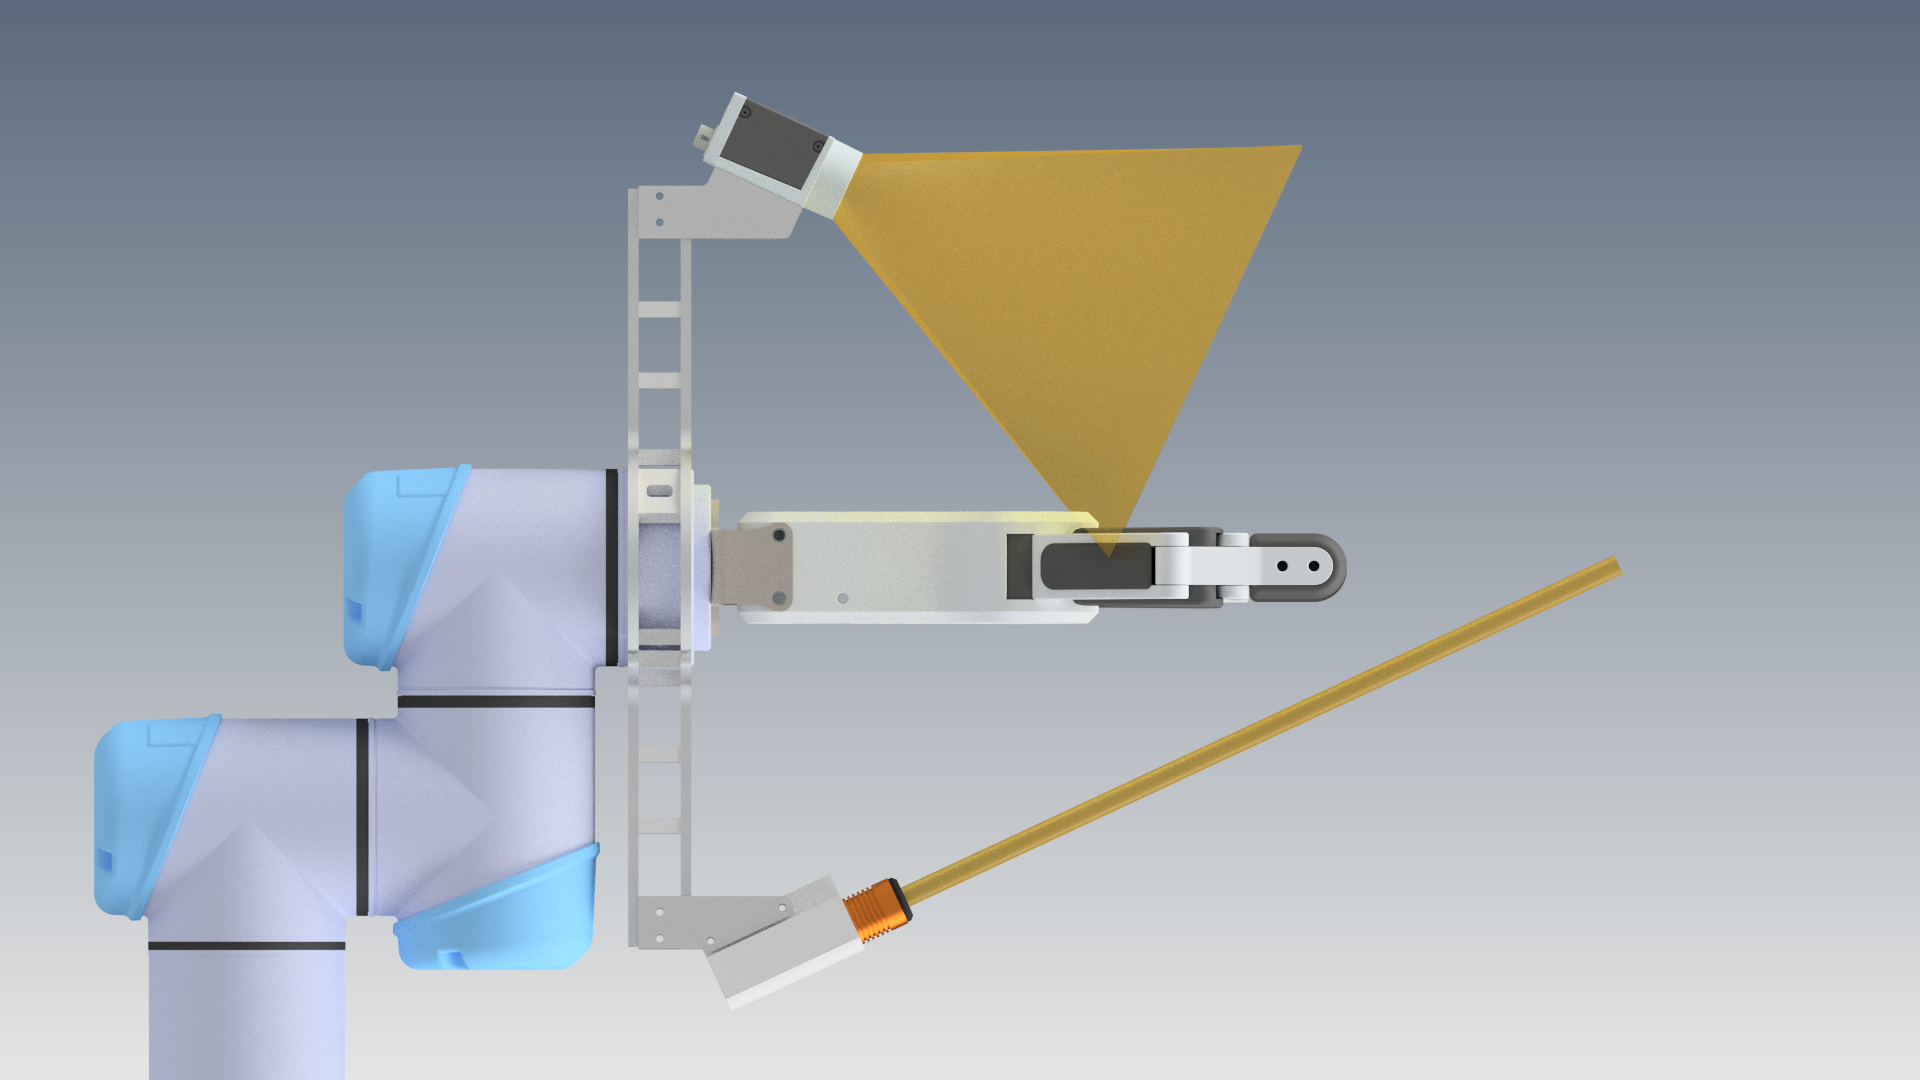
\includegraphics[width=0.45\textwidth]{figures/widok_robot_2.png}
	\centering
	\caption{Widok uchwytu w pionowej płaszczyźnie przekroju}
	\label{fig:widok_robot_2}
\end{figure}

\begin{figure}[ht!]
	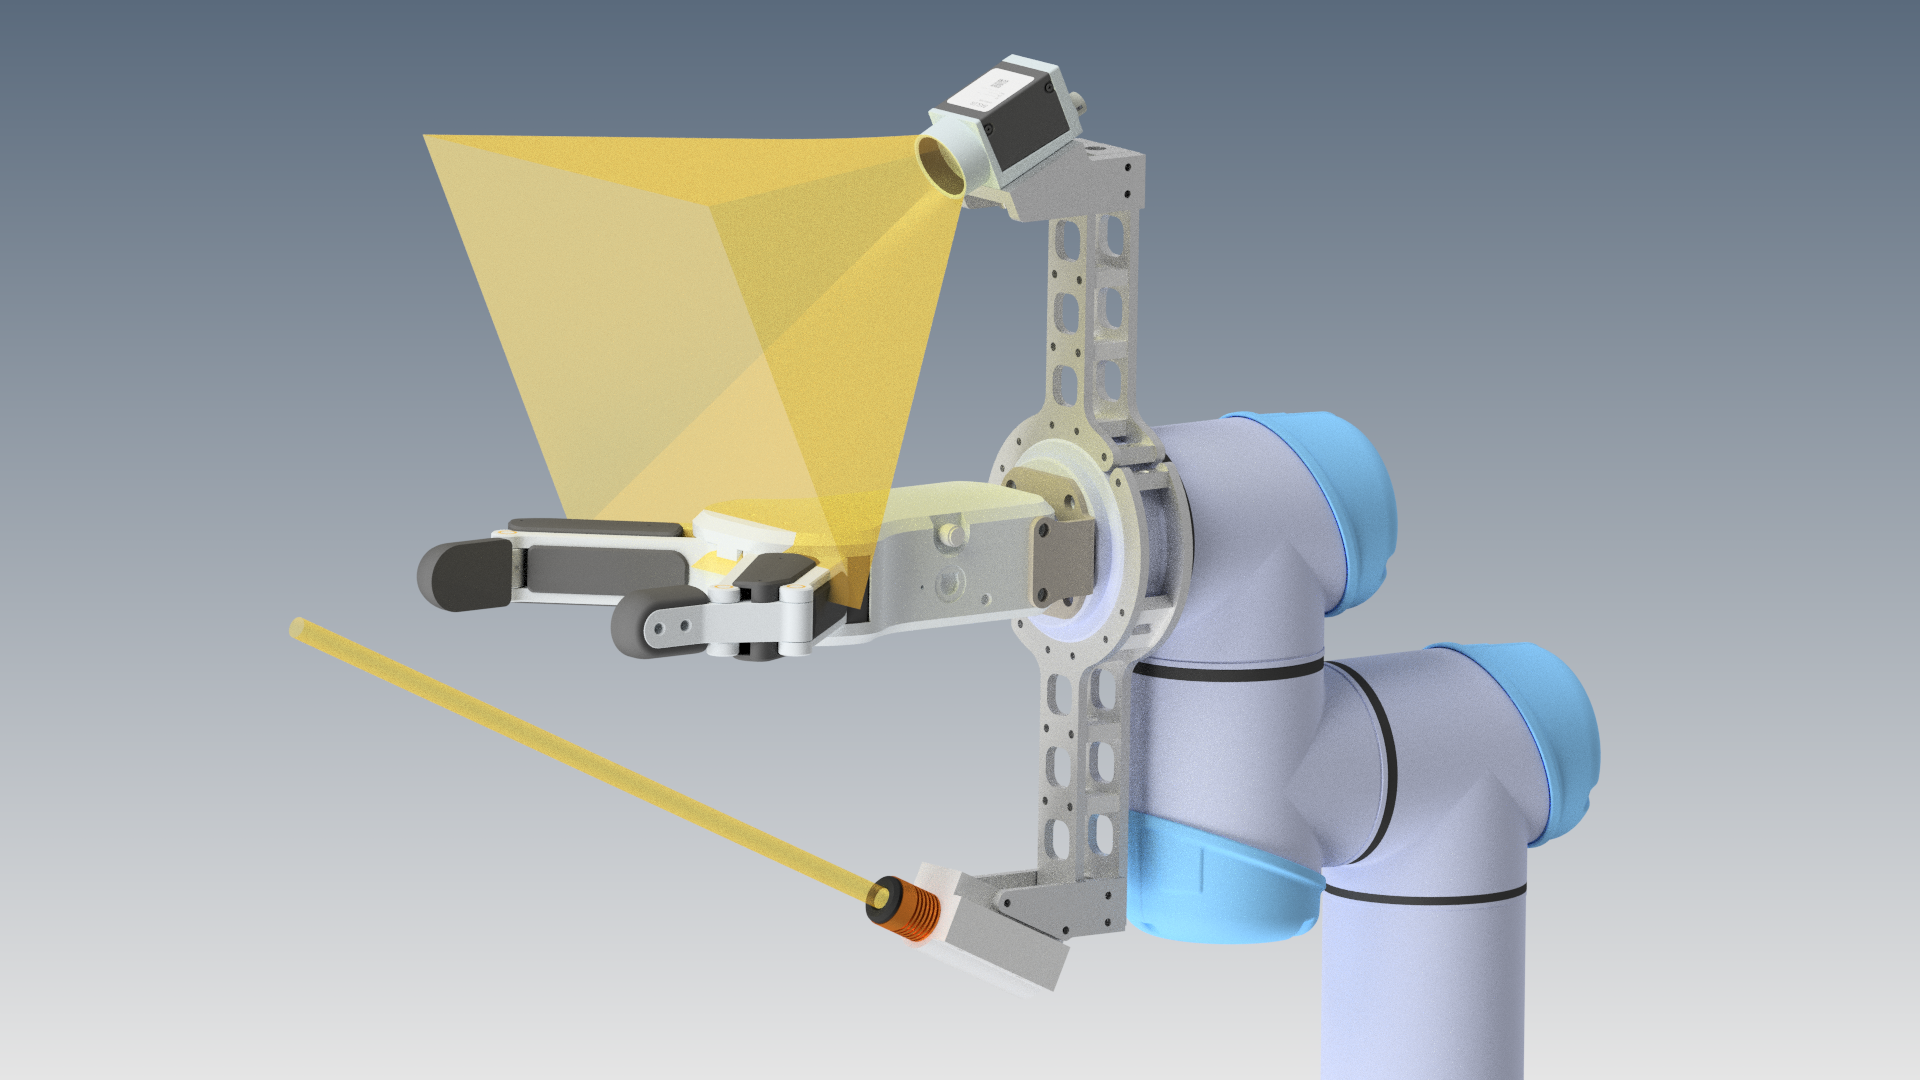
\includegraphics[width=0.45\textwidth]{figures/widok_robot_3.png}
	\centering
	\caption{Widok uchwytu w widoku izometrycznym}
	\label{fig:widok_robot_3}
\end{figure}

Kąt nachylenia obu elementów jest symetryczny względem osi obrotu ostatniego członu ramienia i wynosi dla każdego elementu z osobna 25 stopni (względem osi). W celu modyfikacji (zmniejszenia lub bardziej prawdopodobnego zwiększenia) pola widzenia projektowanego układu konieczne jest przeprojektowanie wyłącznie dwóch elementów.

Mimo, iż elementy mocujące kamerę i laser wykonane zostały z PLA to uzyskana sztywność konstrukcji omawianego uchwytu jest wystarczająca.

Istotną kwestią do rozważenia w dalszych pracach nad projektem jest opracowanie rozwiązania uniemożliwiającego obrót lasera wokół własnej osi. Proponowanym rozwiązaniem, którego nie udało się zaimplementować jest wklejenie wewnątrz obudowy lasera (w podstawie) cienkiej taśmy dwustronnej, która będzie zapobiegać obrotowi lasera. To rozwiązanie należałoby wprowadzić jak najszybciej przy dalszych pracach, ponieważ zapobiegnie ono konieczności wielokrotnego kalibrowania układu kamera-laser po przypadkowym przemieszczeniu lasera, które w aktualnej postaci mocowania jest bardzo łatwo wywołać.

\section{Elektronika}

Jako zasilanie kamery postanowiono wykorzystać przewód Ethernet oraz fakt obsługiwania przez zastosowane urządzenie standardu PoE. Dzięki temu rozwiązaniu do zasilania oraz transmisji danych z kamery wykorzystywany jest tylko jeden przewód.

Zasilanie lasera zostało doprowadzone przez odłączany przewód z wyjściami bananowymi, które służą do zasilania układu z zasilacza laboratoryjnego. W podstawowej konfiguracji konieczne jest doprowadzenie napięcia zasilania lasera 5V oraz masy. Istnieje możliwość sterowania intensywnością oświetlenia generowanego przez laser aczkolwiek do tego zadania konieczne byłoby wykorzystanie układu umożliwiającego płynne regulowanie napięcia w zakresie 0-5V podawanego na jeden z czterech pinów (szczegóły w dokumentacji lasera).

\section{Program - Visual}

Program został napisany w środowisku VisualStudio 2017.

Program wykorzystuje biblioteki:
\begin{itemize}
\item OpenCV v3.4.0
\item Eigen v3.3.3
\item Pylon v5.0
\end{itemize}

Do poprawnego działania algorytmu niezbędne są informacje uzyskane podczas kalibracji kamery zawierające macierz kamery, macierz deformacji oraz równanie płaszczyzny lasera.

\subsection{Kalibracja kamery}

Procedura kalibracji kamery rozpoczyna się od sprawdzenia czy w folderze projektu znajduje się plik z danymi o kalibracji kamery. W przypadku, gdy wspomniany plik nie istnieje program przystępuje do wykonania procedury kalibracji kamery.

Kalibracja wymaga szachownicy kalibracyjnej, której wymiary są zdefiniowane w zmiennych $"checkerboard\_size\_x"$ oraz $"checkerboard\_size\_y"$. 

Do poprawnego wykonania kalibracji konieczne jest pobranie wcześniej zdefiniowanej (przez zmienną $"camera\_calib\_img\_count"$) liczby obrazów zawierających widok na tablicę kalibracyjną w różnych obszarach widzenia kamery (przy różnych przemieszczeniach obrazu lecz bez jego obracania). Pobieranie następuje poprzez wciśnięcie dowolnego klawisza. Po pobraniu obrazów następuje proces kalibracji z wykorzystanie funkcji dostępnej w OpenCV $"calibrateCamera"$. W zależności od liczby pobranych klatek oraz posiadanej mocy obliczeniowej proces ten może trwać co najmniej kilka minut. Po wyznaczeniu parametrów kamery następuje ich zapis do pliku $"cam\_param.yml"$.

\subsection{Wyznaczenie płaszczyzny lasera}

W przypadku, gdy wczytane zostały parametry kamery sprawdzane jest czy istnieje plik zawierający informacje o położeniu płaszczyzny lasera $"PlaneEq.yml"$.

Kalibracja płaszczyzny lasera wymaga szachownicy kalibracyjnej znajdującej się na płaszczyźnie ale nie zajmującej całego obszaru widzianego przez kamerę. Istotne jest to, iż gdy szachownica oświetlona jest laserem, to nie jest rozpoznawana przez algorytm.

Po wciśnięciu klawisza 'p' następuje przechwycenie klatki. Na obrazie następuje wyszukanie szachownicy poprzez funkcję $"calculateCheckerboardVector"$, która to zwraca równanie płaszczyzny tablicy kalibracyjnej względem kamery. Oraz wyszukanie linii lasera $"find\_laser"$ w formie wektora punktów 2D. Następnie wykorzystując równanie płaszczyzny i punkty 2D obliczane jest położenie tych punktów w przestrzeni wykorzystując $"projectImagePointsOntoPlane"$ (funkcja działa na zasadzie opisanej we wstępie). Gdy zebrana jest chmura punktów, można dokonać dopasowania płaszczyzny funkcją $"best\_plane\_from\_points"$. 

Gdy zebrana jest wystarczająca ilość punktów i dokładność płaszczyzny będzie zadowalająca można zapisać plik z równaniem płaszczyzny lasera poprzez przytrzymanie klawisza 's'.
Testowano po 4 krotnym zebraniu punktów i równanie płaszczyzny zostało wyznaczone względnie poprawnie (nie badano dokładności).

\subsection{Skanowanie}

W przypadku, gdy istnieją pliki kalibracyjne kamery oraz płaszczyzny program przechodzi do skanowania. Po wciśnięciu klawisza 'n' pobierany jest obraz, wyszukiwana jest linia lasera, obliczane jest położenie punktów lasera w przestrzeni oraz są one dodawane do chmury punktów. Tak uzyskaną chmurę można zapisać przy pomocy klawisza 's'.

\subsection{projectImagePointsOntoPlane}

Należy zaznaczyć, iż powyższa funkcja, na której opiera się cały program została dostarczona przez Jan Wietrzykowski.

\begin{thebibliography}{00}
\bibitem{b1}Pose Estimation, $https:\/\/docs.opencv.org\/3.3.0\/d7\/d53\/tutorial\_py\_pose.html$, 13.06.2018

\end{thebibliography}

\end{document}
